\chapter{Spreading} % (fold)
\label{cha:spreading}

\section{Which model for news spreading?}

In order to choose a model for the spreading of news or ideas it's necessary to point out
what means in this field an infection, and to interpret the related quantities.
A person "infected'' by a news it's not a person just only reached by the news, but it's a person
who partecipates to the spreading by communicating to its neighbours and potentially infect them.
The decision to spread the information it's an individual choice, expressing the interest
of the person to the news, and indicates the presence of a personal threshold of reaction related to the news or ideas.
The threshold can also be influenced by the neighbourhood or the community membership.


In the epidemic models, such as the SI model, the coefficient $\beta$ represents the rate of trasmission of the infection and it is constant for the whole population, indicating the dependence on the properties of the pathogen.

In the news field $\beta$ can be interpreted as an intrinsic power of trasmission of the news.
This power of trasmission may be associated to the journalistic concept of \textit{newsworthiness},
which includes all the characteristics that make a fact a worthy news.
But the expanding phenomenon of \textit{fake news} shows that the speed of diffusion it's not only related to
the worthiness of an information. A recent paper published on Science \cite{Vosoughi_2018} shows how false news on Twitter spread 
``significantly farther, faster, deeper, and more broadly than the truth in all categories of information''.
The authors of the paper tried to explain the faster speed of diffusion of the false news by its novelty and the conveying
of strongest emotive reactions like surprise or disgust.


A news coverage is usually characterized also by a certain amount of time after which the news naturally ``dies'' out.
%%Considering the meaning assigned to the news infection the people who don't care no more about the news and stops communicating
%%about it 

This fact can be modeled with the SIS formulation where the people recover from the infection with a rate $\mu$.
The coefficient $\mu$, likewise $\beta$, it's constant and in this case can represents the intrinsic property of a news to vanish,
which makes the people stopping communicating about the news.




In order to include also the personal threshold reaction to a news would be necessary to use a more sophisticated model, MILLI

In this chapter we'll describe the results we obtained by applying the \textbf{SI}, \textbf{SIS}, \textbf{SIR},
and \textbf{Threshold} diffusion models both on the crawled data and on the synthetic graphs (Erdős–Rényi and
Barabási–Albert) generated from the original one. In each section, a comparison between the three networks will be
provided along with some details on the implementation of the tests of every model.


\section{SI model} % (fold)
\label{sec:si_model}


\begin{figure}[H]
  \centering
  \begin{subfigure}{0.45\textwidth}
    \resizebox{\textwidth}{!}{
      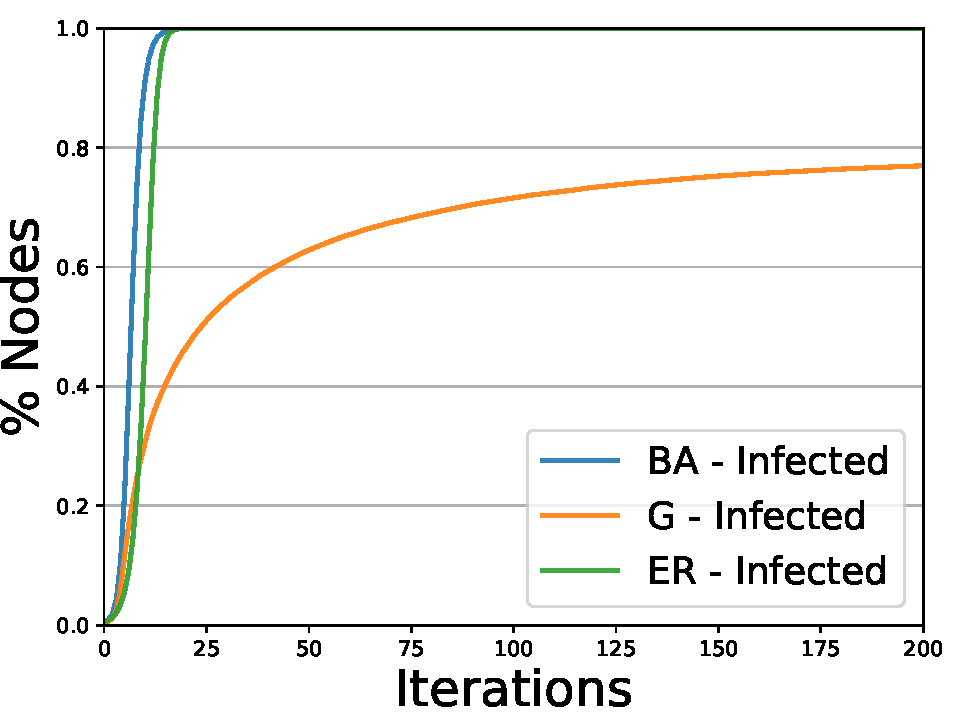
\includegraphics{images/spreading/si/trend_comparison_01.pdf}
    }
            \caption{Infection rate $\beta_0= 0.01$.}
            \label{fig:diff_si_1}
        \end{subfigure}
        \begin{subfigure}{0.45\textwidth}
            \resizebox{\textwidth}{!}{
              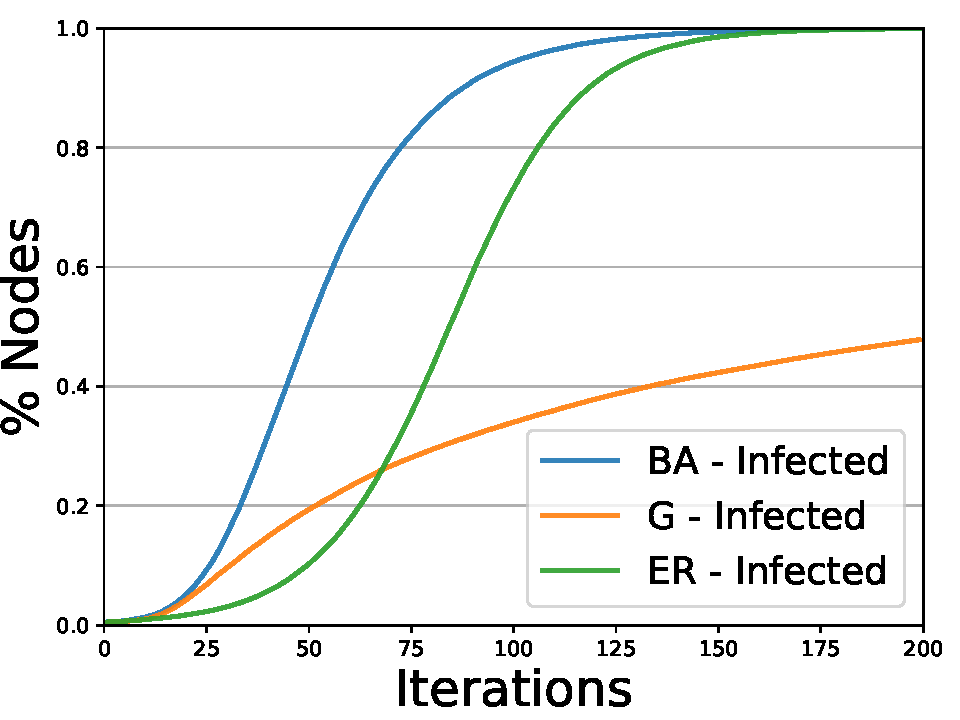
\includegraphics{images/spreading/si/trend_comparison_001.pdf}
            }
            \caption{Infection rate $\beta_1= \frac{\beta_0}{10} =  0.001$. }
            \label{fig:diff_si_2}
          \end{subfigure}
          \caption{Comparison of two trasmission rates in the SI model, for the original network $G$, the Erdos-Renyi $ER$ and the Barabasi-Albert $BA$.}
          \label{fig:diff_si}
     \end{figure}

    For the \textbf{Susceptible-Infected} model we've started with a random $0.005\%$ of the total population ($3$ nodes)
    of each network being infected, representing the earliest sources of information.
    In Fig. \ref{fig:diff_si} we compare two different trasmission rates, with an order of magnitude of difference:
    $ \beta_0 =0.01$ for   $\beta_1 = 0.001$. The original network asymptotically reach the saturation regime only for the fraction of nodes
    in the strong connected component.


% section si_model (end)

\section{SIS model} % (fold)
\label{sec:sis_model}
    \begin{figure}[H]
        \centering
        \begin{subfigure}{0.3\textwidth}
            \resizebox{\textwidth}{!}{
                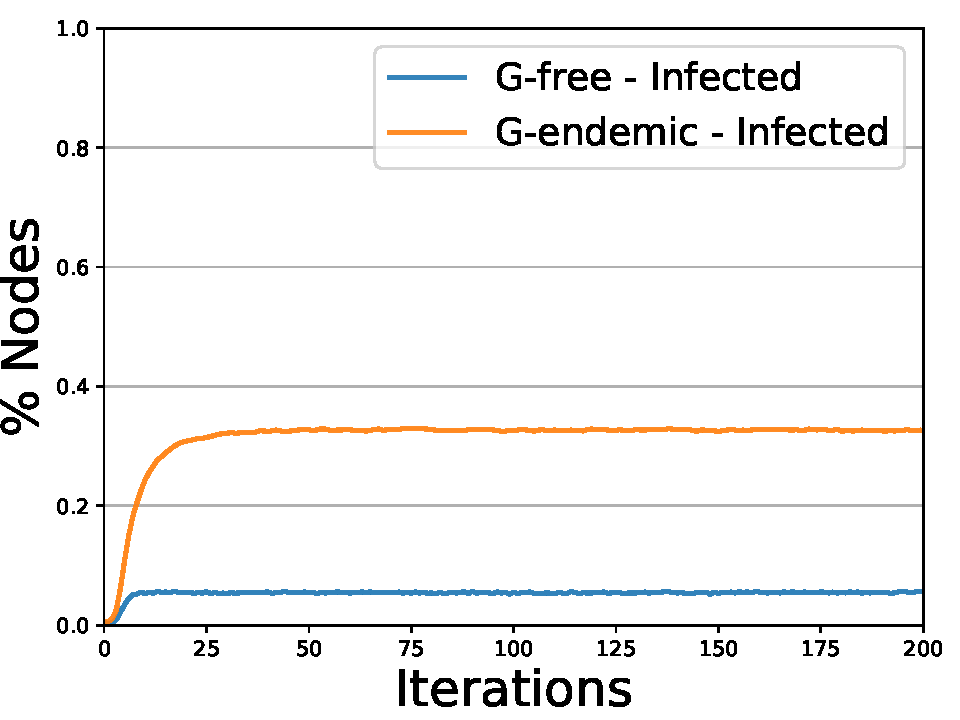
\includegraphics{images/spreading/sis/diffusion_G_comparison.pdf}
            }
            \caption{Original network}
            \label{diff_sis}
        \end{subfigure}
        \begin{subfigure}{0.3\textwidth}
            \resizebox{\textwidth}{!}{
                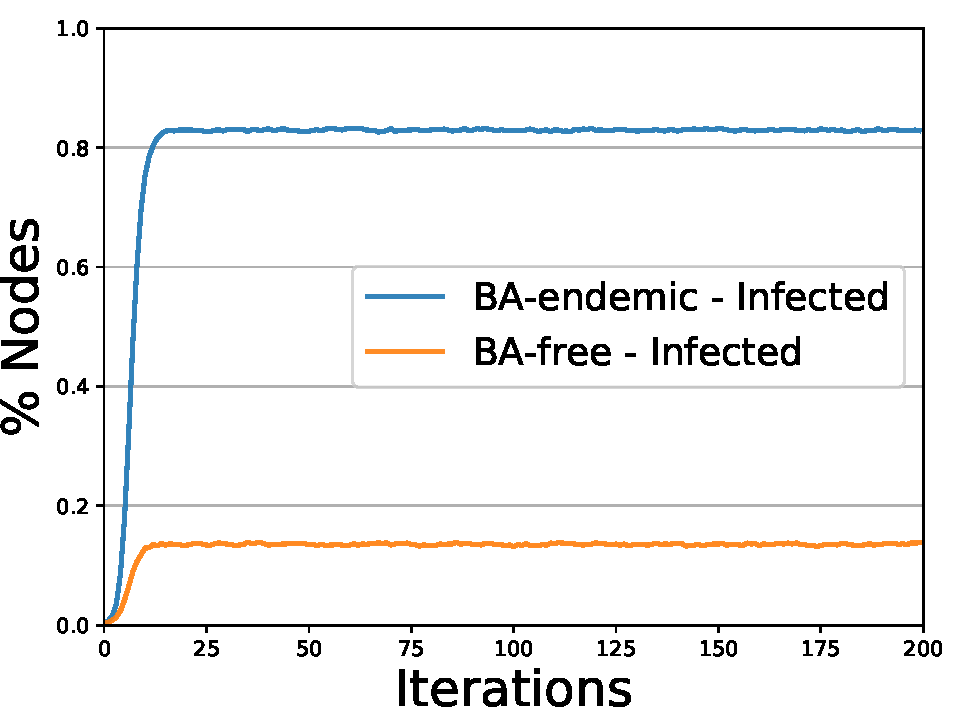
\includegraphics{images/spreading/sis/diffusion_BA_comparison.pdf}
            }
            \caption{Barabasi-Albert network}
            \label{diff_sis_er}
        \end{subfigure}
        \begin{subfigure}{0.3\textwidth}
            \resizebox{\textwidth}{!}{
                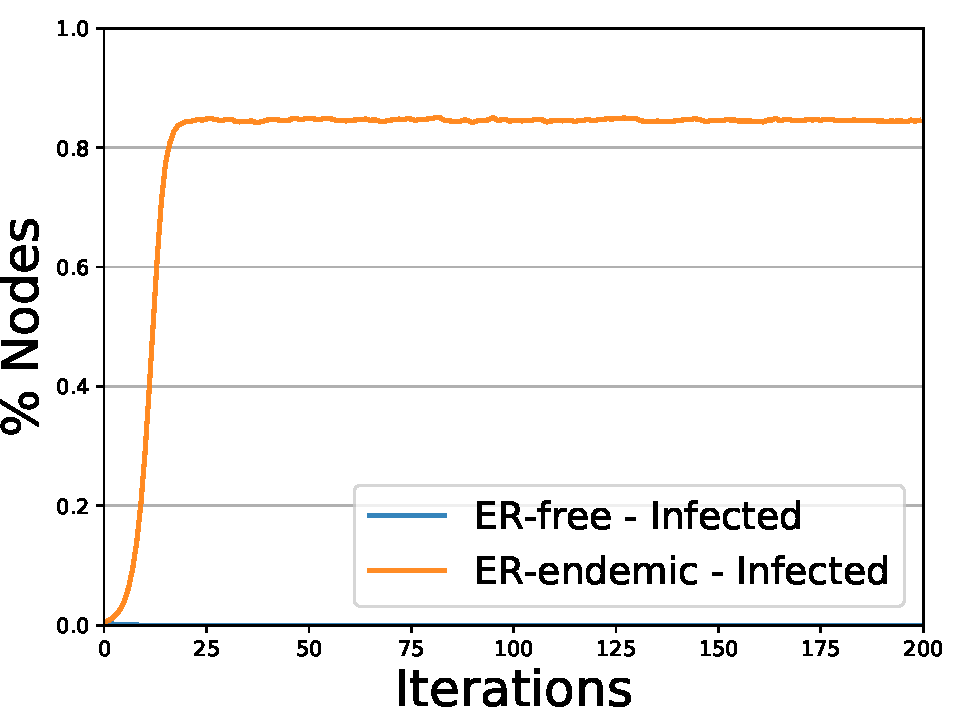
\includegraphics{images/spreading/sis/diffusion_ER_comparison.pdf}
            }
            \caption{Erdos-Renyi network}
            \label{diff_sis_ba}
        \end{subfigure}
        \caption{Comparison of the SIS model for the original network $G$, the Erdos-Renyi $ER$ and the Barabasi-Albert $BA$.}
        \label{fig:diff_sis_comparison}
      \end{figure}

      The introduction of the recovery rate $\mu$ in the \textbf{Susceptible-Infected-Susceptible} model for networks epidemics
      provides an epidemic threshold $\lambda_C$ for the spreading rate $\lambda$, dependent on the second order moment of the degree
      distribution $\langle k^2 \rangle$.
      For a random network the epidemic threshold given by Eq. \ref{eq:epidemic_threshold} is finite, and defines two possible asymptotically outcomes, an \textbf{endemic state} characterized by a finite fraction of infected individuals, and a completely \textbf{disease free} state.
      \begin{equation}
        \lambda_C(ER) = \frac{1}{\langle k \rangle +1 } \Rightarrow \lambda>\lambda_C:\: \text{epidemic state}
        \label{eq:epidemic_threshold}
      \end{equation}
      The free-scale networks are characterized by a diverging variance, which means the epidemic threshold tends to vanish, causing a finite fraction of infected individuals also for small $\lambda$. 
      We used the random network threshold to choose the recovery rate to simulate both the possible states. We observe in Fig. \ref{fig:diff_sis_comparison} how for the free-scale networks the infected fraction is always finite, below and above the epidemic threshold, while for the random network we observe also the disease free state.
      
% section sis_model (end)

\section{SIR model} % (fold){}
\label{sec:sir_model}
    The key characteristic of the \textbf{Susceptible-Infected-Recovered} model consists in the possibility
    of the individuals to recover from the disease and hence to be ``removed'' from the population instead of returning to the susceptible state.
    We have tested this model either for the case in which $\mu$ is smaller than $\beta$ and the other way around. The graphs representing this different situations for all the three networks are visible in Fig. \ref{fig:diff_sir_total}.

    \begin{figure}
        \begin{subfigure}{0.45\textwidth}
            \resizebox{\textwidth}{!}{
                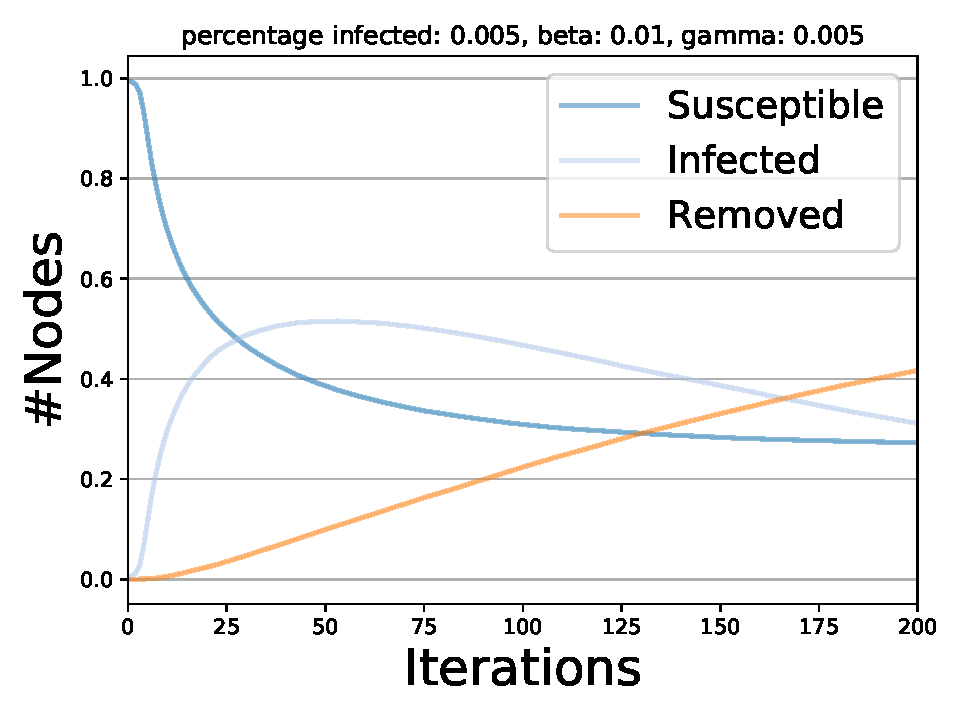
\includegraphics{images/spreading/sir/diffusion_smaller.pdf}
            }
            \caption{Original network}
            \label{diff_sir_smaller}
        \end{subfigure}
        \begin{subfigure}{0.45\textwidth}
            \resizebox{\textwidth}{!}{
                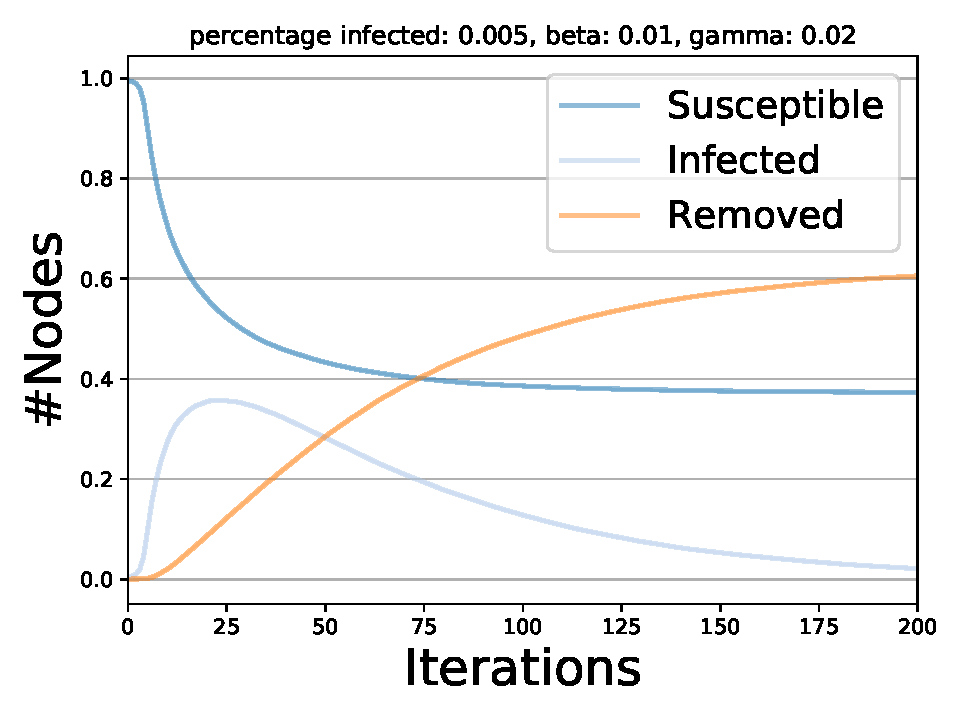
\includegraphics{images/spreading/sir/diffusion_greater.pdf}
            }
            \caption{Original network}
            \label{diff_sir_greater}
        \end{subfigure}
        \begin{subfigure}{0.45\textwidth}
            \resizebox{\textwidth}{!}{
                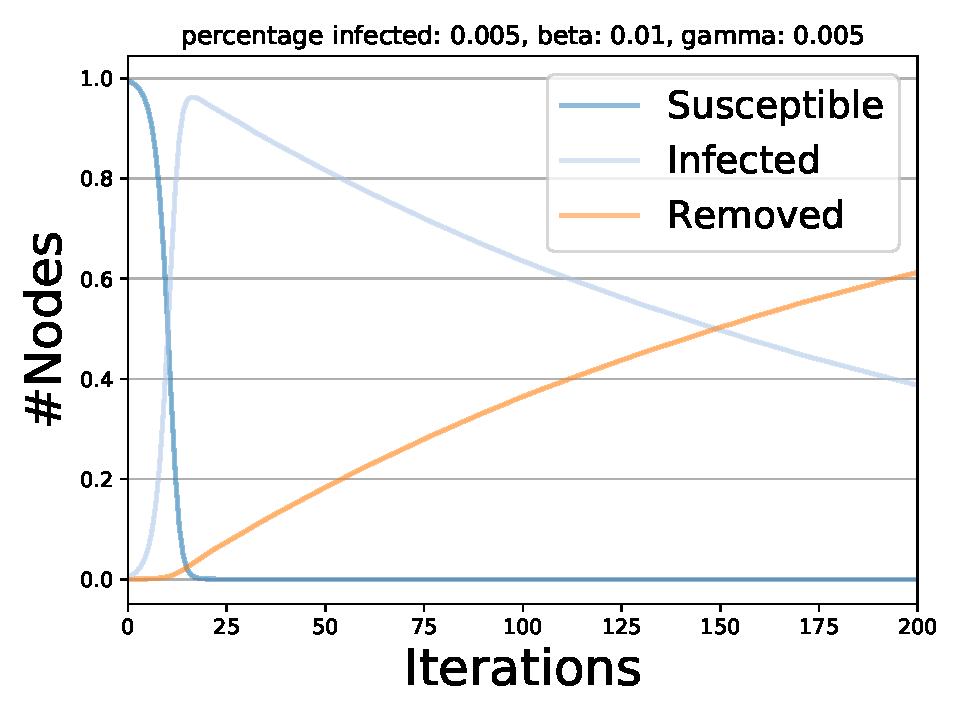
\includegraphics{images/spreading/sir/diffusion_er_smaller.pdf}
            }
            \caption{Erdos-Renyi network.}
            \label{diff_sir_er_smaller}
        \end{subfigure}
        \begin{subfigure}{0.45\textwidth}
            \resizebox{\textwidth}{!}{
                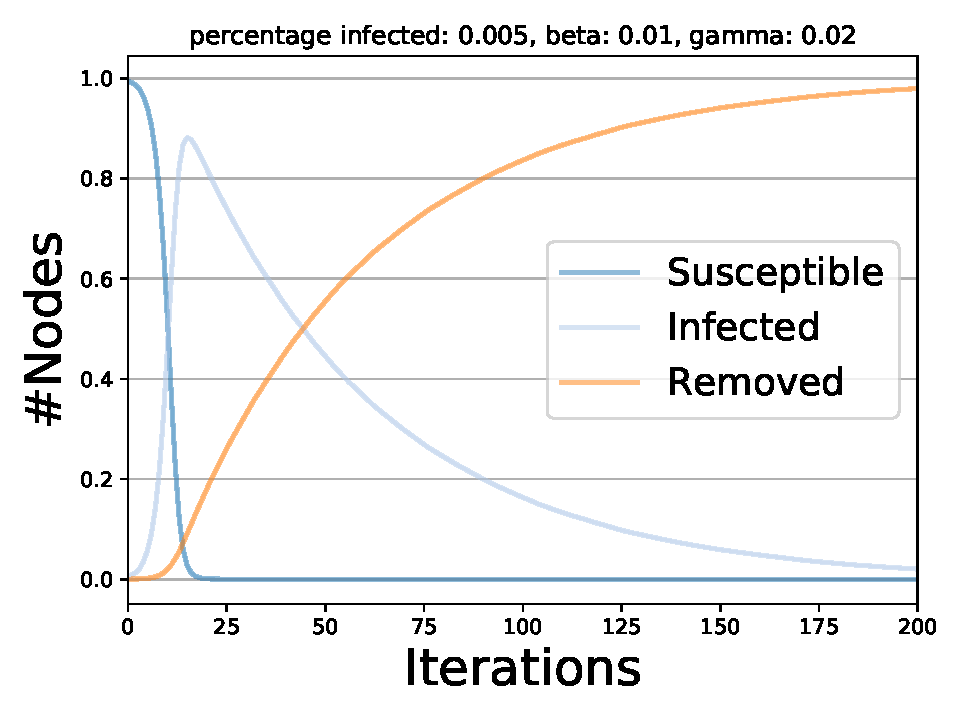
\includegraphics{images/spreading/sir/diffusion_er_greater.pdf}
            }
            \caption{Erdos-Renyi network.}
            \label{diff_sir_er_greater}
        \end{subfigure}
        \begin{subfigure}{0.45\textwidth}
            \resizebox{\textwidth}{!}{
                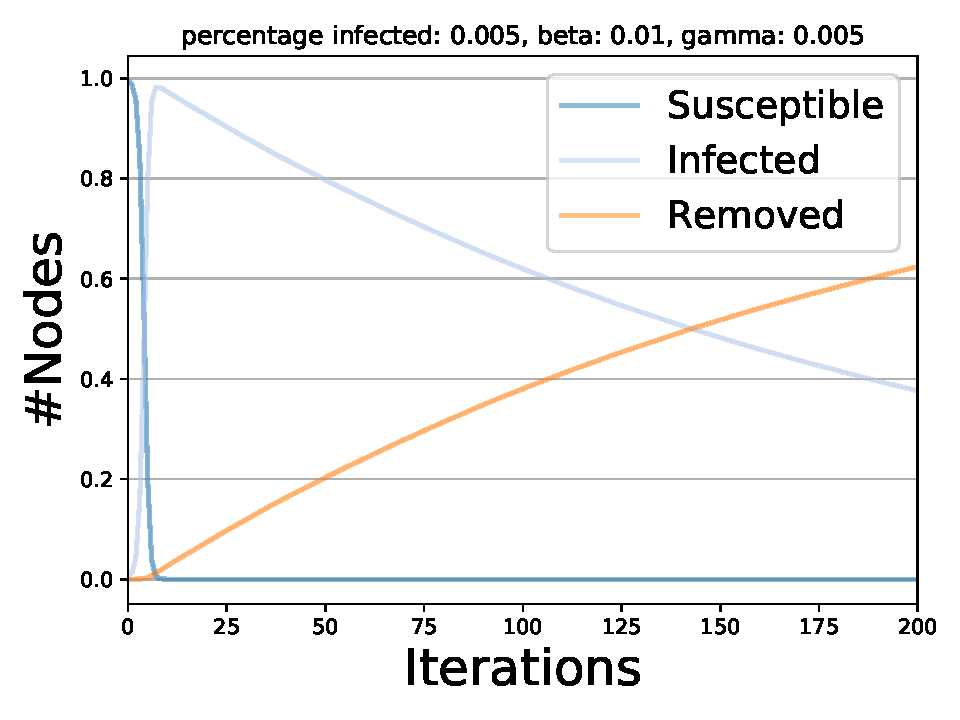
\includegraphics{images/spreading/sir/diffusion_ba_smaller.pdf}
            }
            \caption{Barabasi-Albert network.}
            \label{diff_sir_ba_smaller}
        \end{subfigure}
        \begin{subfigure}{0.45\textwidth}
            \resizebox{\textwidth}{!}{
                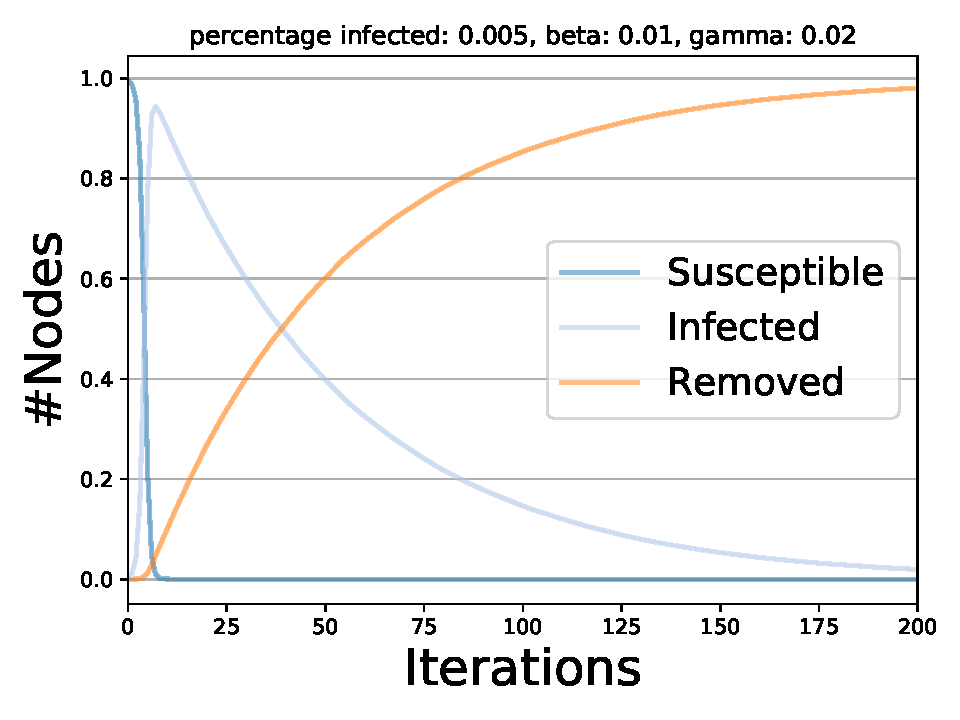
\includegraphics{images/spreading/sir/diffusion_ba_greater.pdf}
              }
            \caption{Barabasi-Albert network.}
            \label{diff_sir_ba_greater}
        \end{subfigure}
        \caption{}
        \label{fig:diff_sir_total}
    \end{figure}

% section sir_model (end)

\section{Threshold model} % (fold)
\label{sec:threshold_model}
    Finally we describe the application of the \textbf{Threshold model} both on the original network and the
    synthetic ones. In order to test this model we've choosen to apply a threshold $\tau$ eguals to $0.10$, the
    diffusion of the infection for this model is represented in Figure \ref{diff_thr_total}. As we can see, for the
    original network we have that almost all the nodes become infected within the first $20$ model's iterations,
    due to the fact that the value choosen for the threshold results to be sufficient for the spreading of the
    infection. If we change the threshold's value, this time using $0.20$, we can observe that the
    original network become immune to the infection, thanks to its internal structure. We can observe
    the same immunity in the Erdős–Rényi and Barabási–Albert network for the original threshold's value.
    \begin{figure}[H]
        \centering
        \begin{subfigure}{0.33\textwidth}
            \resizebox{\textwidth}{!}{
                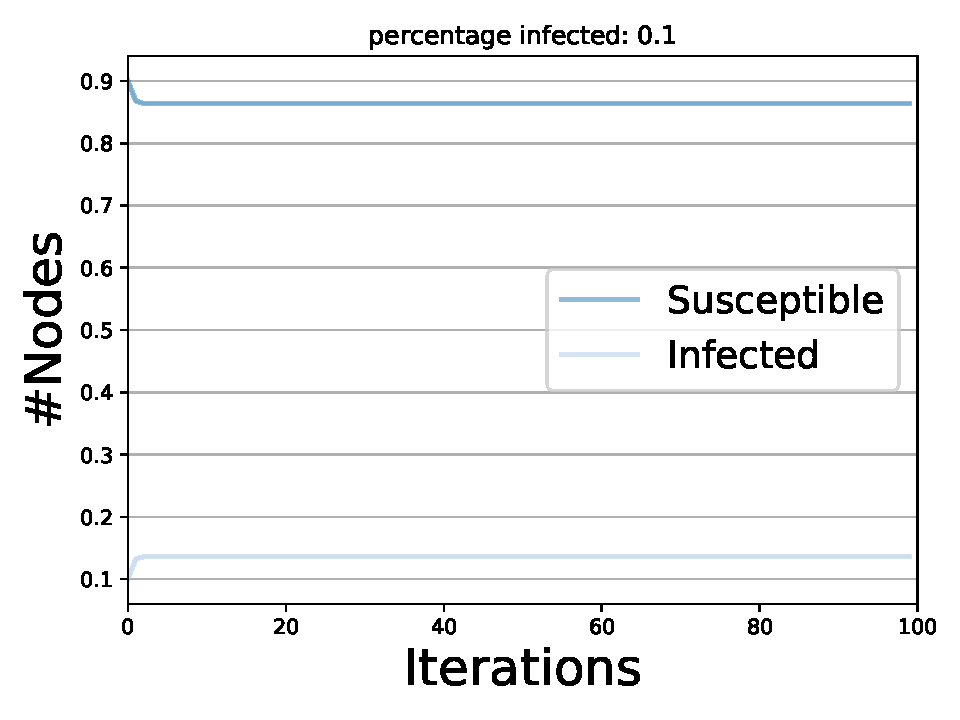
\includegraphics{images/spreading/threshold/diffusion.pdf}
            }
            \caption{}
            \label{diff_thr}
        \end{subfigure}
        \begin{subfigure}{0.33\textwidth}
            \resizebox{\textwidth}{!}{
                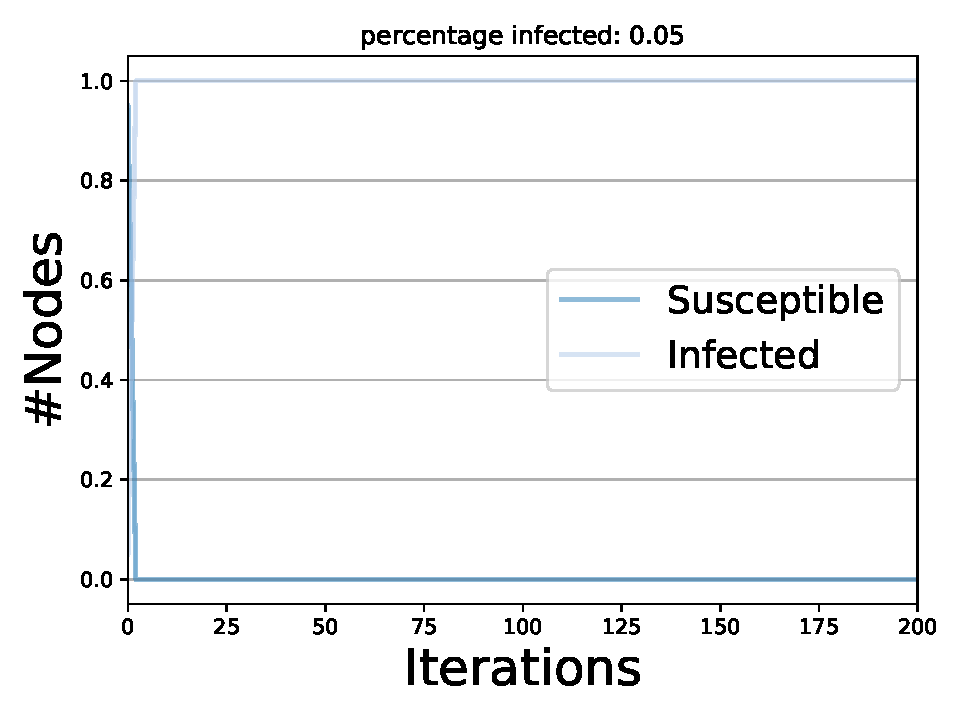
\includegraphics{images/spreading/threshold/diffusion_er.pdf}
            }
            \caption{}
            \label{diff_thr_er}
        \end{subfigure}
        \begin{subfigure}{0.33\textwidth}
            \resizebox{\textwidth}{!}{
                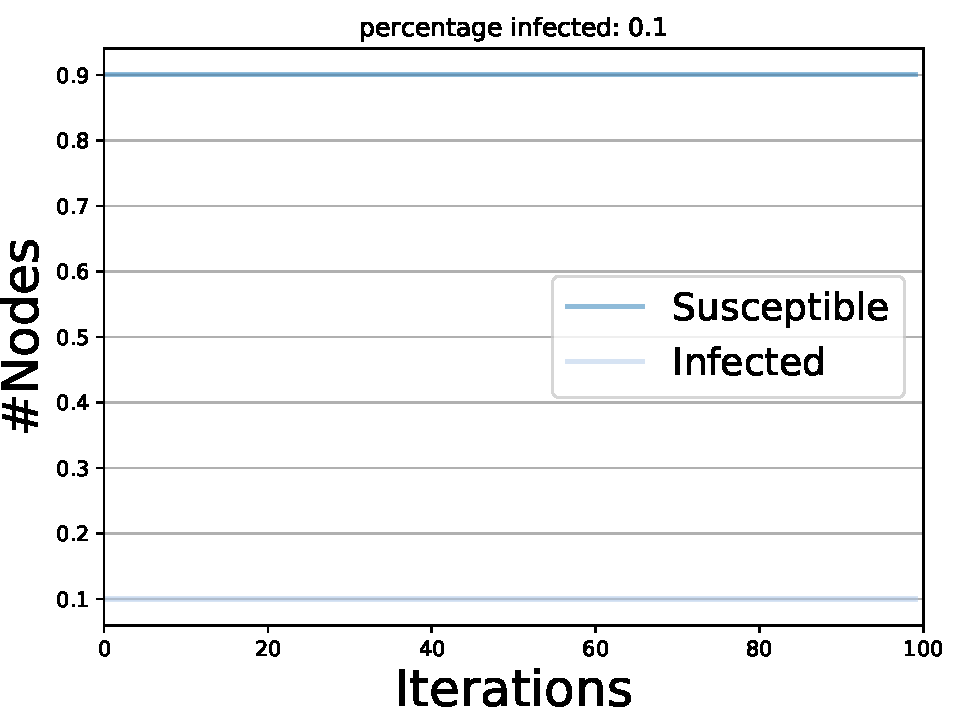
\includegraphics{images/spreading/threshold/diffusion_ba.pdf}
            }
            \caption{}
            \label{diff_thr_ba}
        \end{subfigure}
        \begin{subfigure}{0.33\textwidth}
            \resizebox{\textwidth}{!}{
                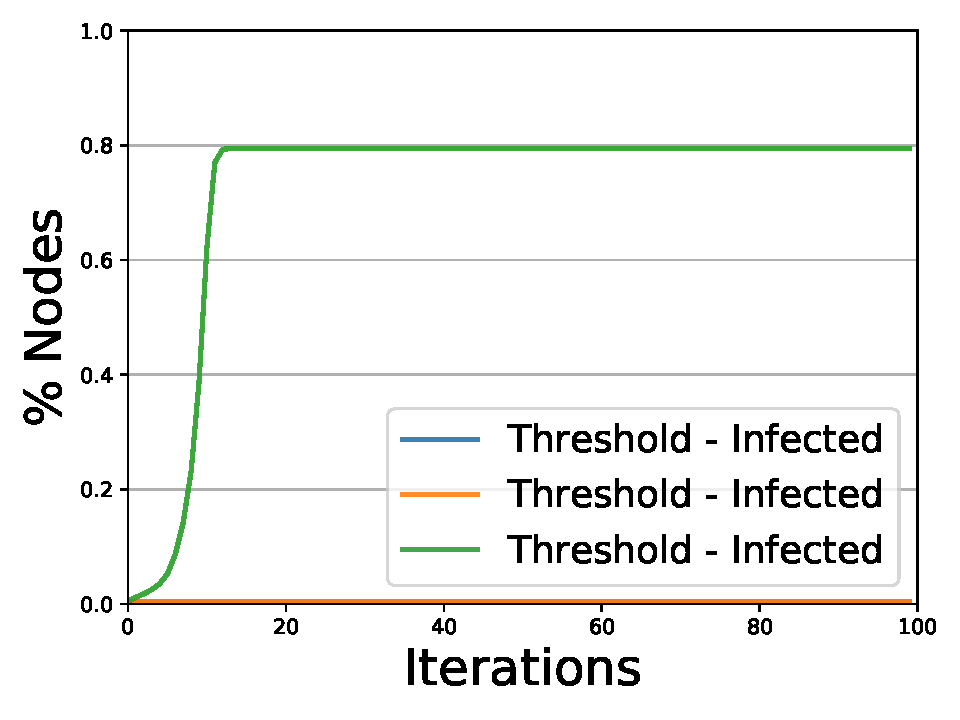
\includegraphics{images/spreading/threshold/trend_comparison.pdf}
            }
            \caption{}
            \label{diff_thr_comparison}
        \end{subfigure}
        \caption{In Figure \ref{diff_thr} is represented the diffusion of the infection for the original network,
        while in Figure \ref{diff_thr_er} and \ref{diff_thr_ba} are represented the cases for the Erdős–Rényi and
        the Barabási–Albert network, respectively. A comparison between the three networks is represented in Figure
        \ref{diff_thr_comparison}.}
        \label{diff_thr_total}
    \end{figure}

% section threshold_model (end)

\section{The New York Times vs La Repubblica }

Idea: let's start with the same news, but two different nodes, there is a big difference in diffusion?
Prevision: no, the difference it's minimal because of the presence of hubs.





    
% chapter spreading (end)
